\subsubsection*{Informazioni sul package}
\begin{figure}[h]
	\centering
	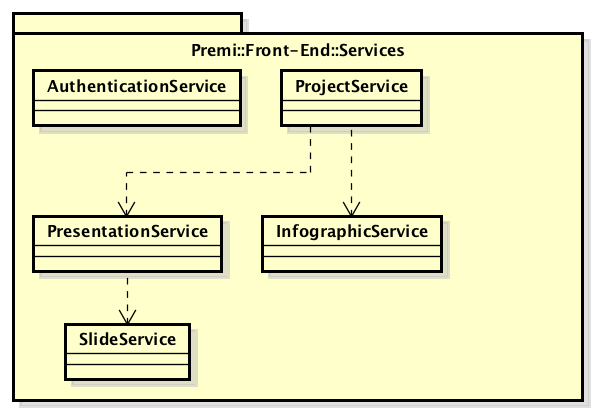
\includegraphics[width=0.9\linewidth]{img/front-end_services}
	\caption[Premi::Front-End::Services]{Premi::Front-End::Services}
\end{figure}
Il package contiene gli elementi per creare i service del \gls{front-end}, ovvero per creare gli oggetti che consentono di interfacciarsi con le API \gls{REST} del \gls{back-end}, popolare il model del client e richiedere l'esecuzione di altre operazioni necessarie al server.

\subsubsection*{Classi contenute}
\begin{itemize}

    \item Premi::Front-End::Services::AuthenticationService:
	\begin{itemize}
		\item \textbf{Descrizione}: classe per la gestione dell'autenticazione e della registrazione di un utente.
	\end{itemize}

    \item Premi::Front-End::Services::ProjectService:
	\begin{itemize}
		\item \textbf{Descrizione}: classe per la gestione di un progetto e dei suoi componenti (presentazione e infografiche).
	\end{itemize}

    \item Premi::Front-End::Services::PresentationService:
	\begin{itemize}
		\item \textbf{Descrizione}: classe per la gestione di una presentazione e dei suoi dati.
	\end{itemize}

    \item Premi::Front-End::Services::SlideService:
	\begin{itemize}
		\item \textbf{Descrizione}: classe per la gestione di una slide, della sua modifica e degli elementi presenti in essa.
	\end{itemize}

    \item Premi::Front-End::Services::InfographicService:
	\begin{itemize}
		\item \textbf{Descrizione}: classe per la gestione di una infografica e della sua modifica.
	\end{itemize}

\end{itemize}
